\documentclass[10pt]{beamer}
\usetheme[
%%% options passed to the outer theme
%    hidetitle,           % hide the (short) title in the sidebar
%    hideauthor,          % hide the (short) author in the sidebar
%    hideinstitute,       % hide the (short) institute in the bottom of the sidebar
%    shownavsym,          % show the navigation symbols
%    width=2cm,           % width of the sidebar (default is 2 cm)
%    hideothersubsections,% hide all subsections but the subsections in the current section
%    hideallsubsections,  % hide all subsections
    left               % right of left position of sidebar (default is right)
%%% options passed to the color theme
%    lightheaderbg,       % use a light header background
  ]{AAUsidebar}

%\usetheme{Berkeley}
%\usefonttheme{serif}
% If you want to change the colors of the various elements in the theme, edit and uncomment the following lines
% Change the bar and sidebar colors:
%\setbeamercolor{AAUsidebar}{fg=red!20,bg=red}
%\setbeamercolor{sidebar}{bg=red!20}
% Change the color of the structural elements:
%\setbeamercolor{structure}{fg=red}
% Change the frame title text color:
%\setbeamercolor{frametitle}{fg=blue}
% Change the normal text color background:
%\setbeamercolor{normal text}{bg=gray!10}
% ... and you can of course change a lot more - see the beamer user manual.

\usepackage{styles/zhfontcfg}
\usepackage[utf8]{inputenc}
\usepackage[english]{babel}
\usepackage[T1]{fontenc}
% Or whatever. Note that the encoding and the font should match. If T1
% does not look nice, try deleting the line with the fontenc.
\usepackage{helvet}

\graphicspath{{AAUgraphics/}}   

% colored hyperlinks
\newcommand{\chref}[2]{%
  \href{#1}{{\usebeamercolor[bg]{AAUsidebar}#2}}%
}
\title[Face Detection]% optional, use only with long paper titles
{\Huge Face Detection}

%\subtitle{副标题}  % could also be a conference name

\date{\today}

\author[赵海伟\  戴嘉伦\  王如晨] % optional, use only with lots of authors
{
  赵海伟\ 戴嘉伦\ 王如晨
 %\href{mailto:jkn@es.aau.dk}{{\tt jkn@es.aau.dk}}
}
% - Give the names in the same order as they appear in the paper.
% - Use the \inst{?} command only if the authors have different
%   affiliation. See the beamer manual for an example

\institute[
%  {\includegraphics[scale=0.2]{aau_segl}}\\ %insert a company, department or university logo
OUC
] % optional - is placed in the bottom of the sidebar on every slide
{% is placed on the title page
CVBIOUC\\
\url{http://vision.ouc.edu.cn/~zhenghaiyong}
  %there must be an empty line above this line - otherwise some unwanted space is added between the university and the country (I do not know why;( )
}


% specify a logo on the titlepage (you can specify additional logos an include them in 
% institute command below

\pgfdeclareimage[height=1.5cm]{titlepagelogo}{AAUgraphics/oucwu.png} % placed on the title page

%\pgfdeclareimage[height=1.5cm]{titlepagelogo2}{graphics/oucwu.png} % placed on the title page
\titlegraphic{% is placed on the bottom of the title page
  \pgfuseimage{titlepagelogo}
%  \hspace{1cm}\pgfuseimage{titlepagelogo2}
}




\begin{document}
% the titlepage
{\aauwavesbg%
\begin{frame}[plain,noframenumbering] % the plain option removes the sidebar and header from the title page
  \titlepage
\end{frame}
}


%%%%%%%%%%%%%%%%

% TOC
\begin{frame}{Agenda}{}
\tableofcontents
\end{frame}
%%%%%%%%%%%%%%%%

\section{Introduction}

\begin{frame}
    \frametitle{Introduction}
   \begin{figure}[!ht]
   \centering
   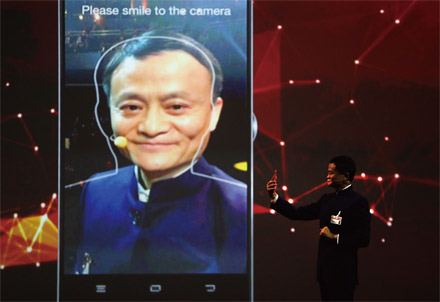
\includegraphics[width=3.0in]{shualian.jpg}
   \end{figure}
   \centering \Large Face Recognition System
\end{frame}

\begin{frame}
    \frametitle{Introduction}
   \large Face Recognition System:
   \begin{figure}[!ht]
   \centering
   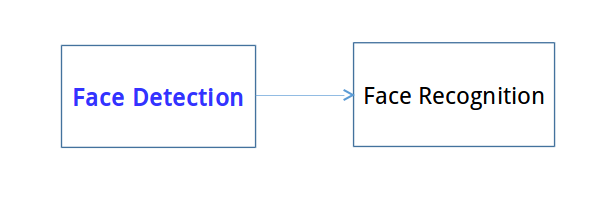
\includegraphics[width=3.2in]{face_recognition.png}
   \end{figure}
\end{frame}



\subsection{Purpose}
\begin{frame}
    \frametitle{Purpose}
   The \underline{\textbf{goal}} of face detection is to determine \underline{\textbf{whether}} or not there are any faces in the image and, if present, return the image \underline{\textbf{location and extent}} of each face\footnote{M. -H. Yang \textit{et al.}, "Detecting Faces in Images: A Survey", PAMI, 2002}.
\end{frame}

\begin{frame}
    \frametitle{Purpose} 
   \begin{figure}[!ht]
   \centering
   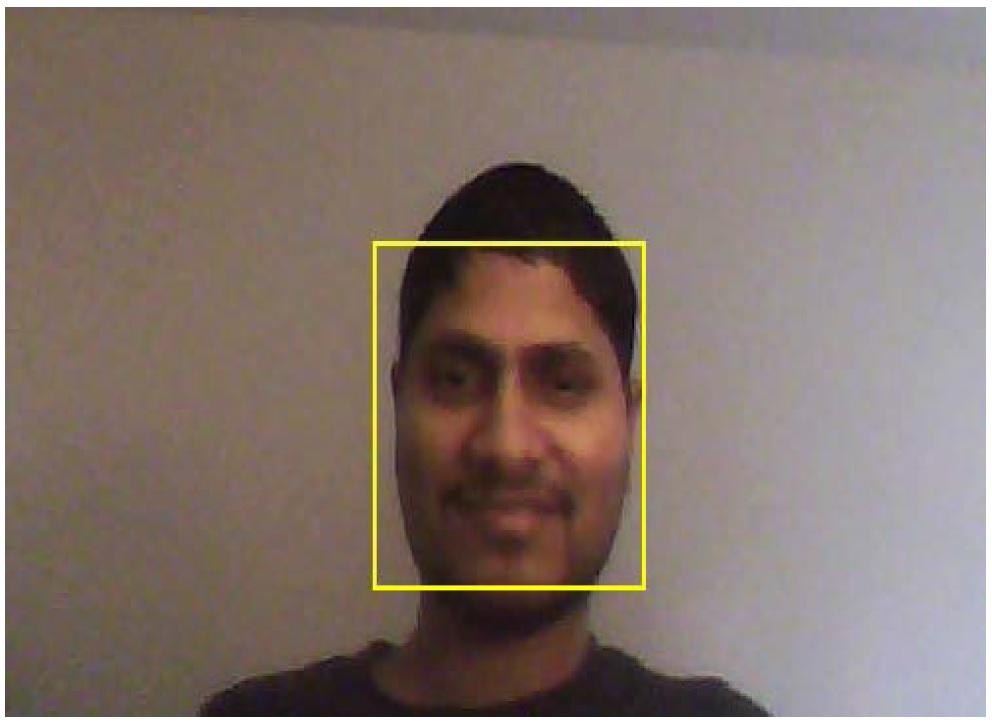
\includegraphics[width=2.8in]{face.jpg}
   \end{figure}
\end{frame}

%\begin{frame}
%    \frametitle{Introduction}
%   \begin{figure}[!ht]
%   \centering
%   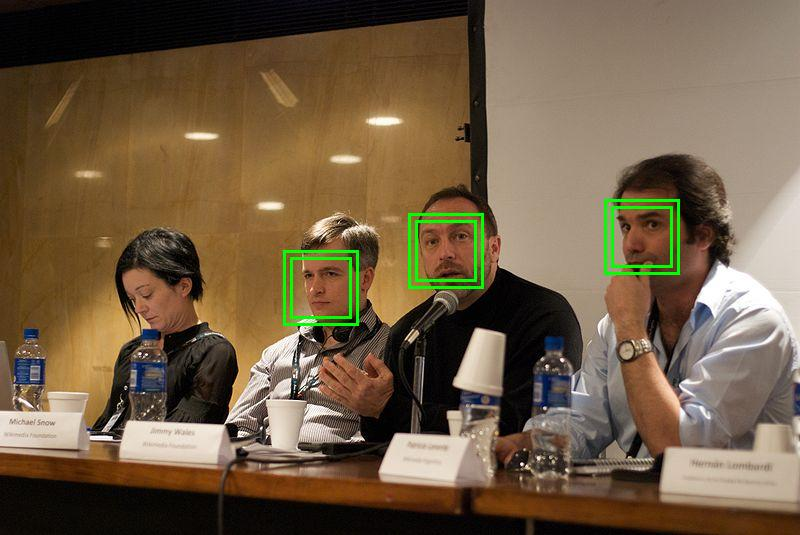
\includegraphics[width=3.0in]{Face_detection.jpg}
%   \end{figure}
%\end{frame}


\subsection{Applications}

\begin{frame}
    \frametitle{Applications}
   \begin{itemize}
   \item Verification\footnote{Subrat Kumar Rath \textit{et al.}, "A Survey on Face Detection and Recognition Techniques in Different Application Domain", MECS, 2014}
   \begin{figure}[!ht]
   \centering
   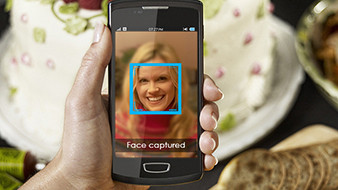
\includegraphics[width=3.0in]{verification.jpg}
   \end{figure}
   \end{itemize}
\end{frame}

\begin{frame}
    \frametitle{Applications}
   \begin{itemize}
   \item Identification
   \begin{figure}[!ht]
   \centering
   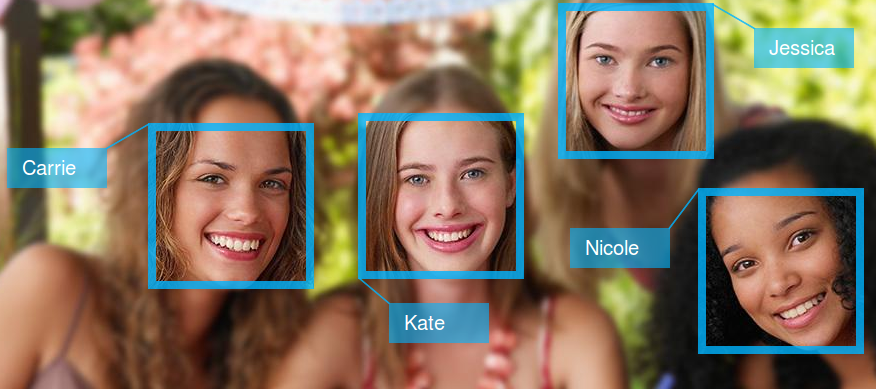
\includegraphics[width=3.0in]{recognition.png}
   \end{figure}
   \end{itemize}
\end{frame}


\begin{frame}
    \frametitle{Applications}
   \begin{itemize}
   \item Face Search
   \begin{figure}[!ht]
   \centering
   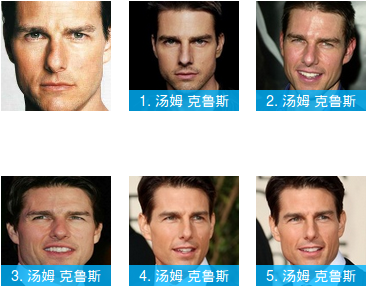
\includegraphics[width=2.5in]{facesearch.png}
   \end{figure}
   \end{itemize}
\end{frame}

\begin{frame}
    \frametitle{Applications}
   \begin{itemize}
   \item Face Track
   \begin{figure}[!ht]
   \centering
   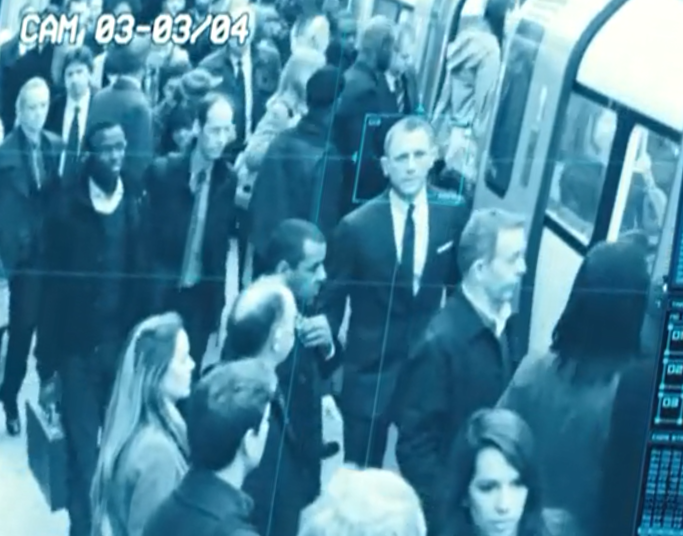
\includegraphics[width=2.5in]{video.png}
   \end{figure}
   \end{itemize}
\end{frame}


\subsection{Challenges}
\begin{frame}
    \frametitle{Challenges}
   \begin{itemize}
   \item Pose\footnote{M.-H. Yang \textit{et al.}, "Detecting Faces in Images: A Survey", PAMI, 2002}
   \end{itemize}
     \begin{figure}
     \begin{minipage}[t]{0.18\linewidth} 
    \centering 
     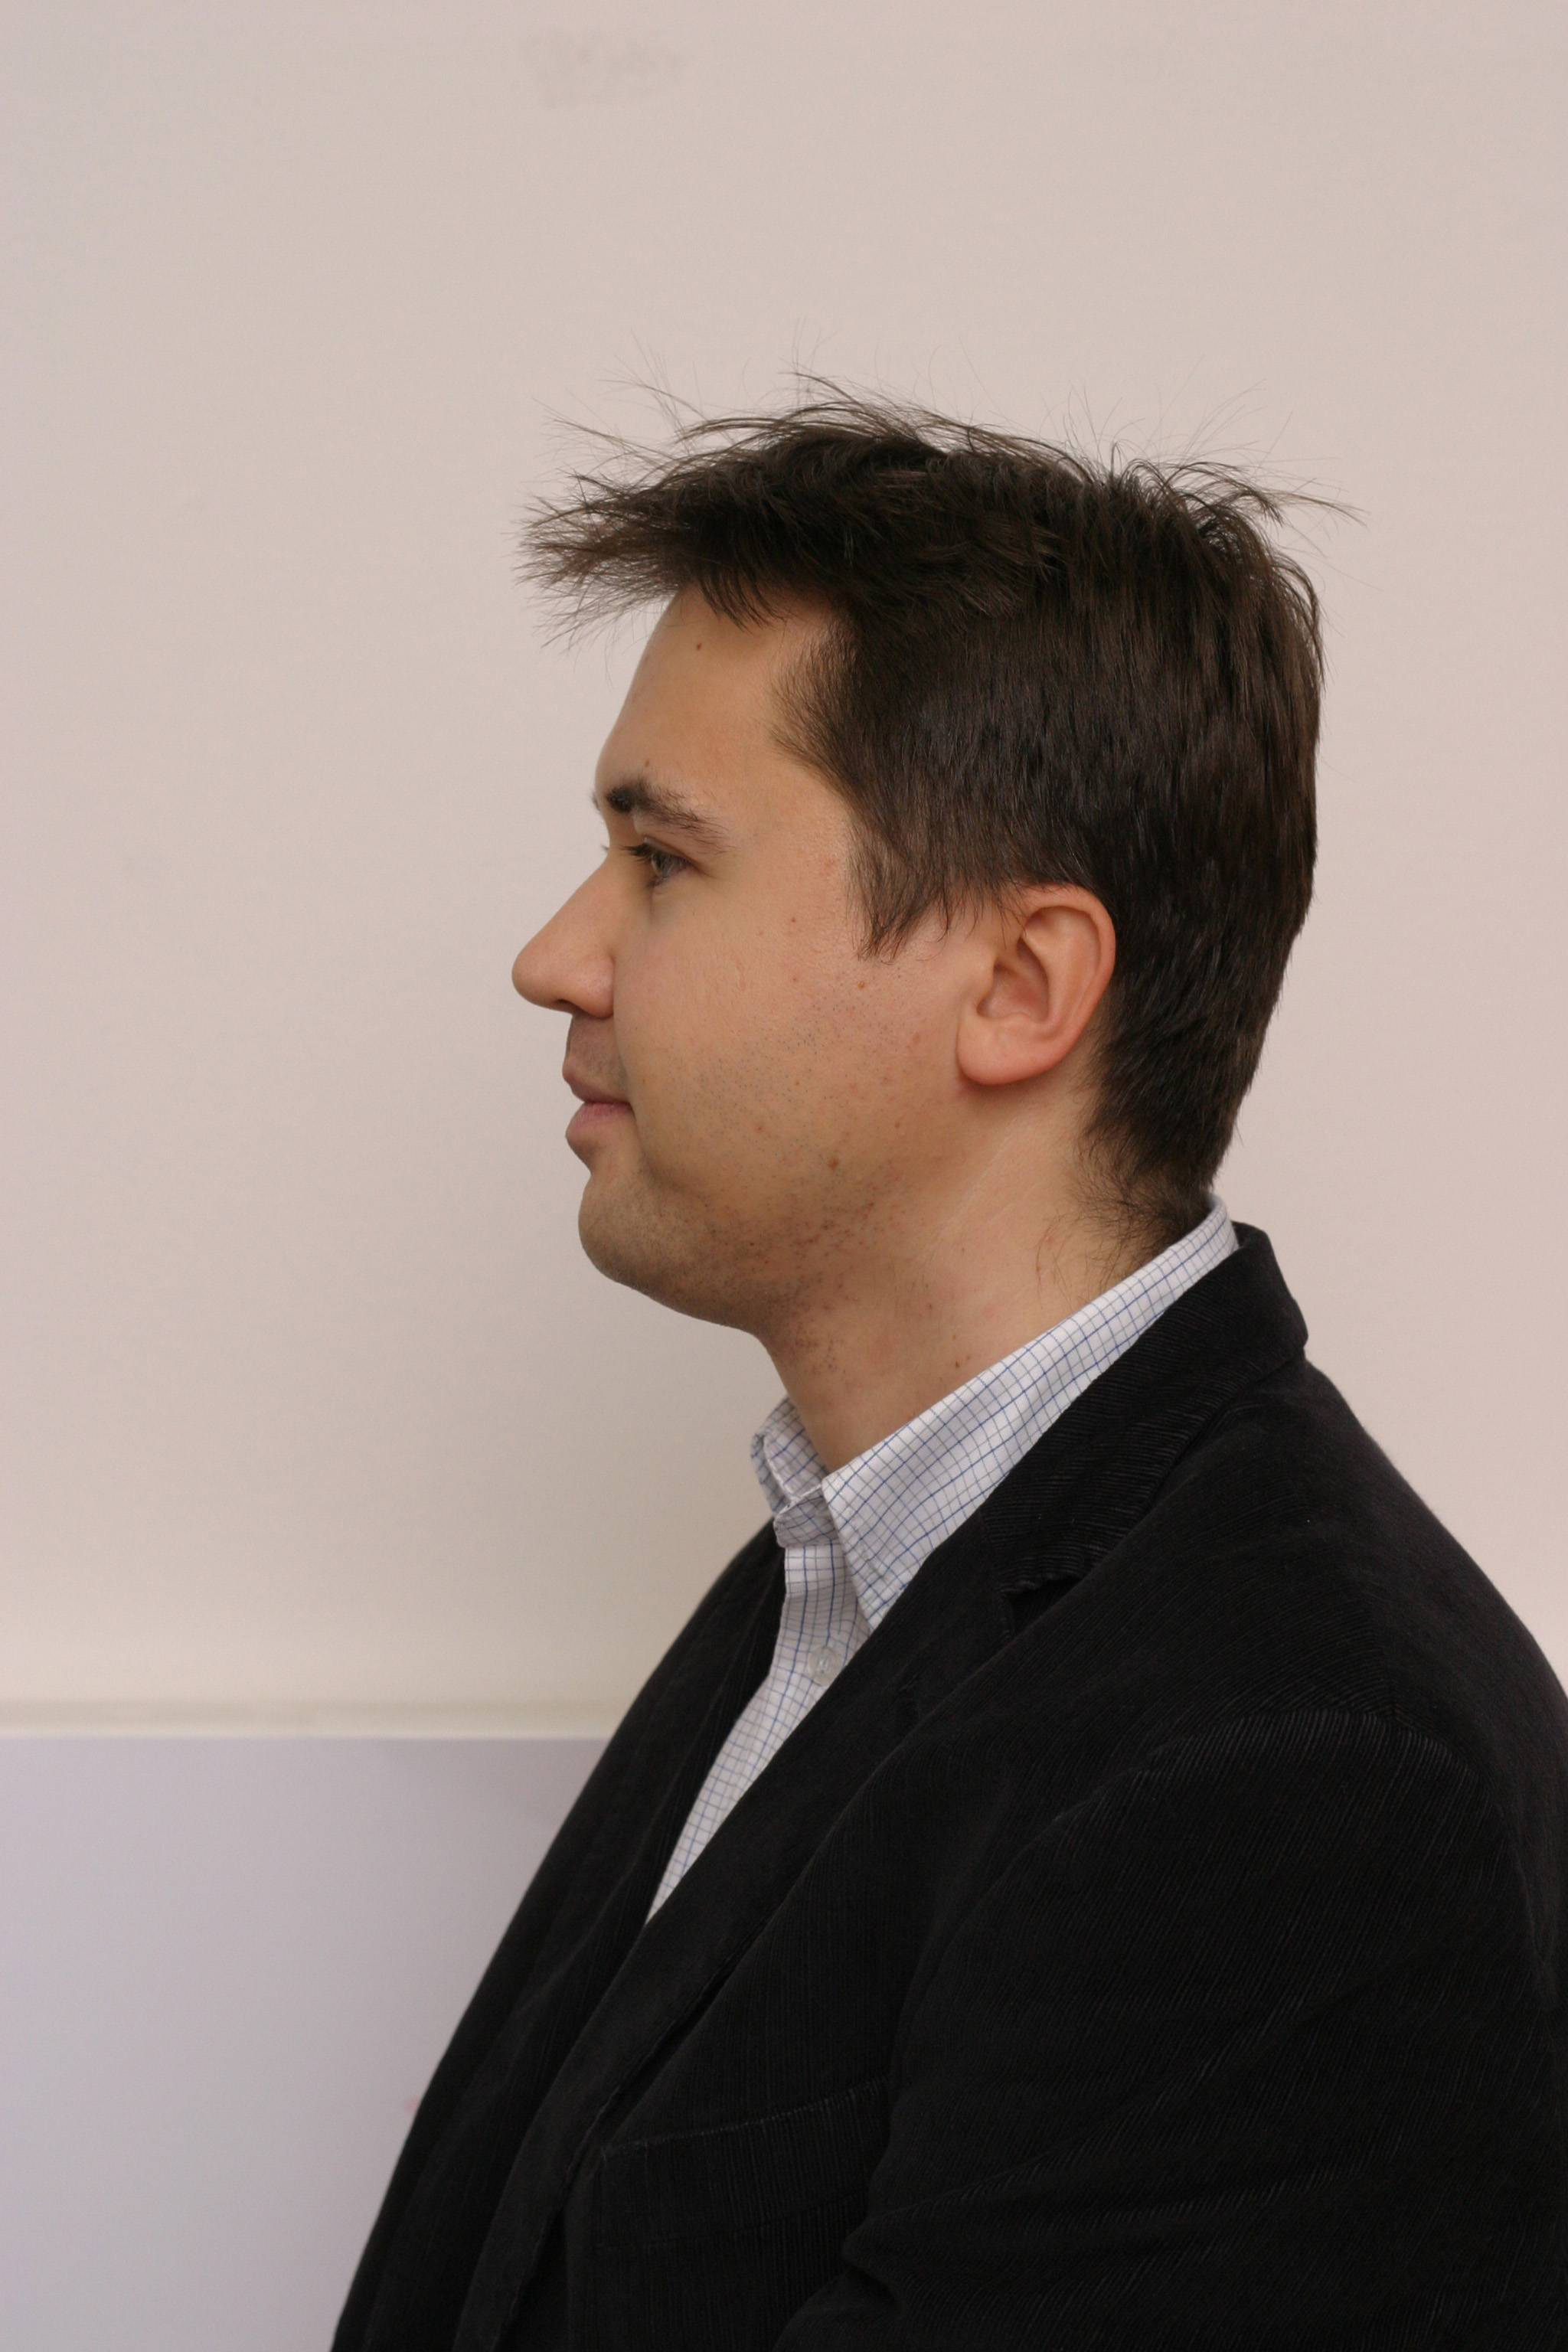
\includegraphics[width=0.7in]{d1.jpg} 
   \end{minipage}
   \begin{minipage}[t]{0.18\linewidth} 
     \centering 
     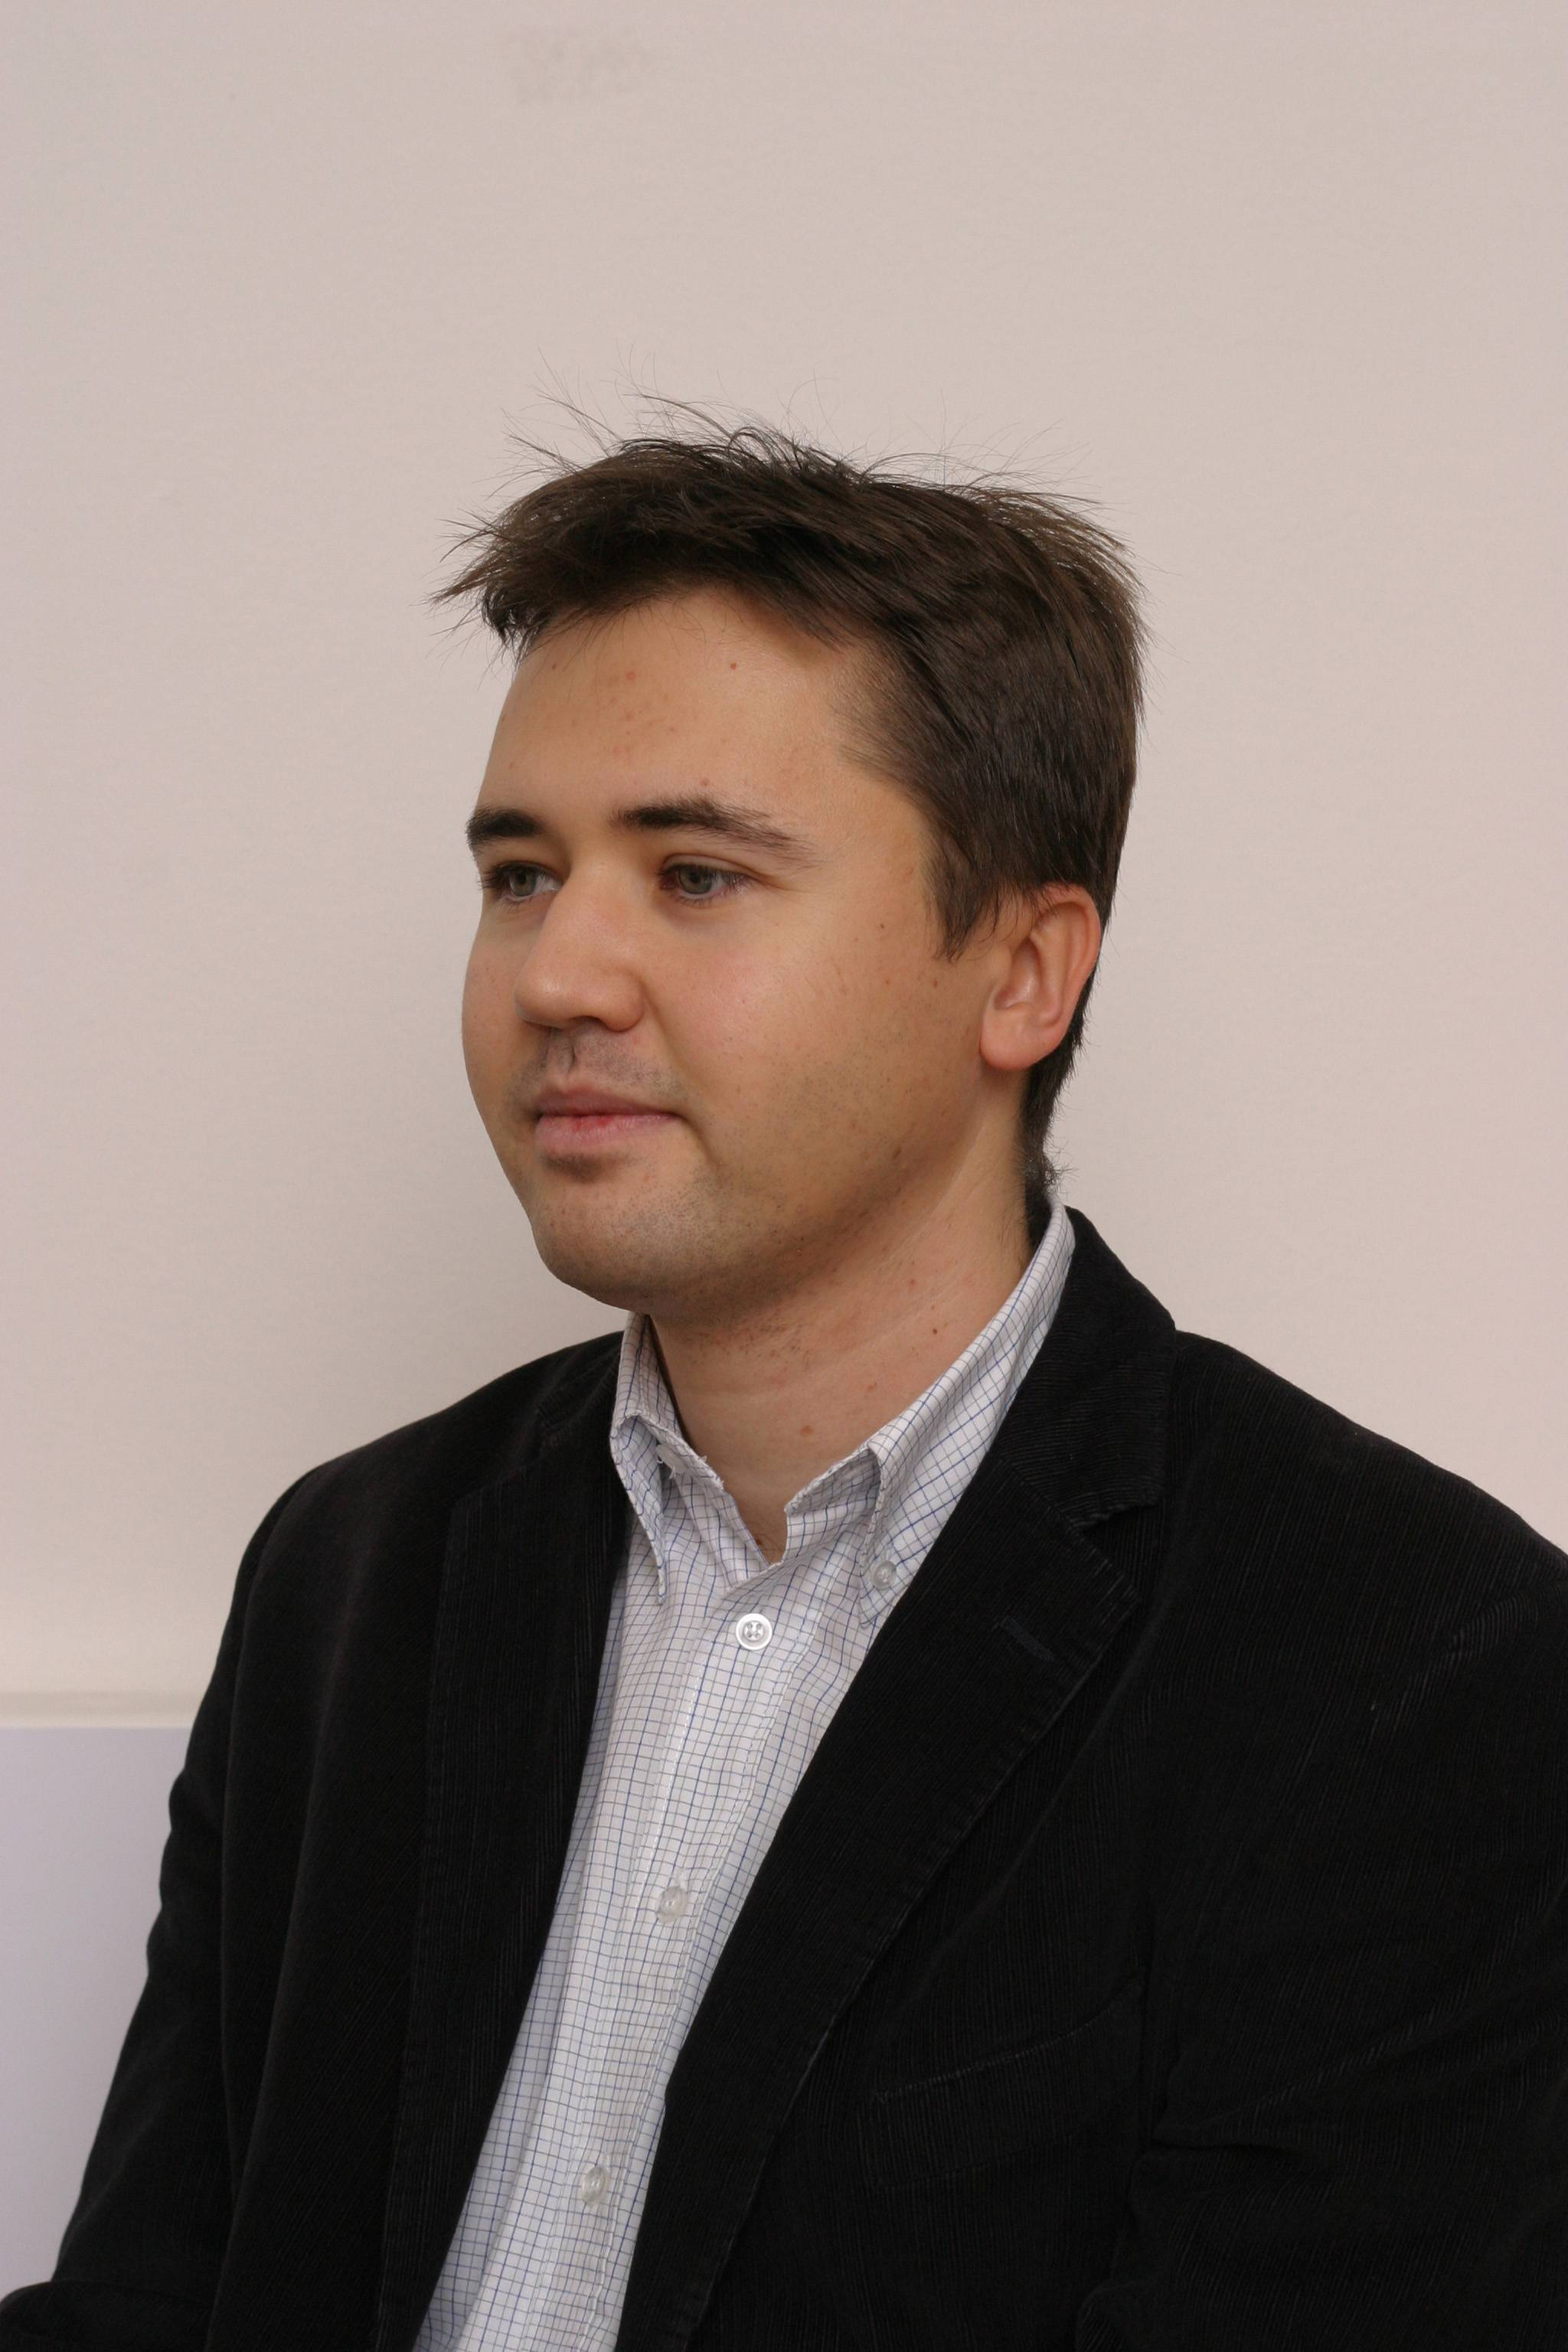
\includegraphics[width=0.7in]{d2.jpg} 
   \end{minipage} 
   \begin{minipage}[t]{0.18\linewidth} 
     \centering 
   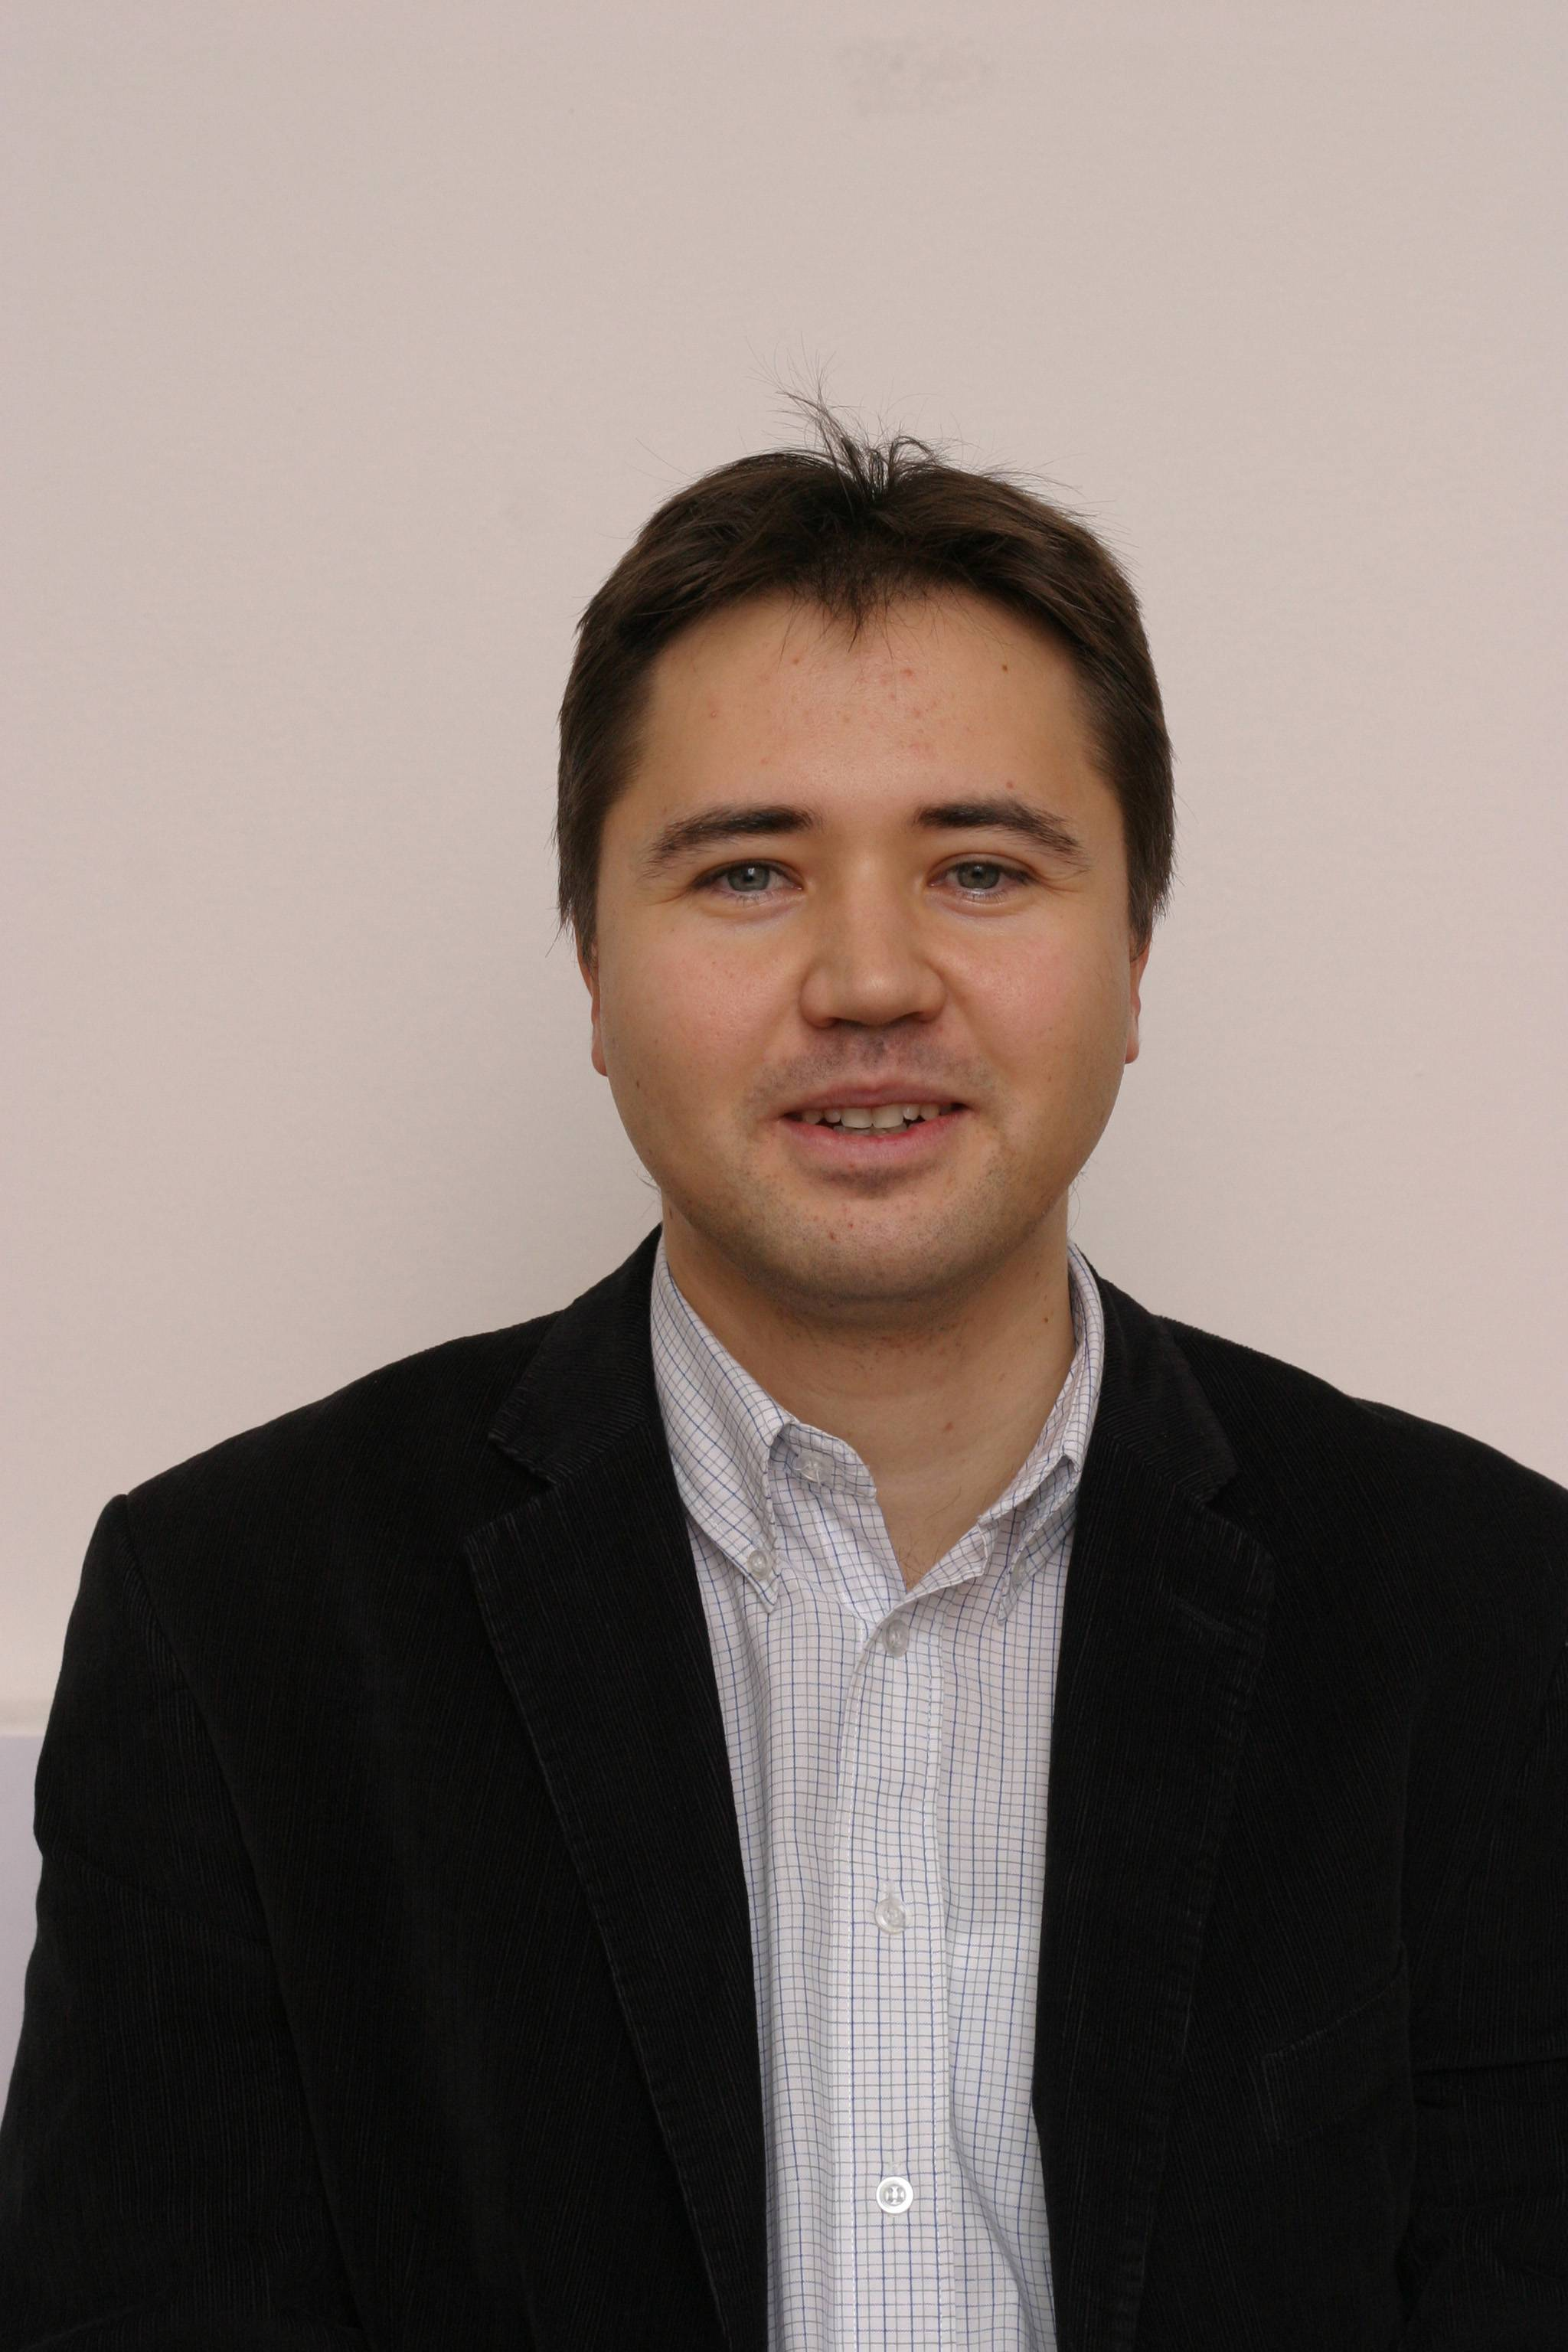
\includegraphics[width=0.7in]{d3.jpg} 
   \end{minipage}
   \begin{minipage}[t]{0.18\linewidth} 
     \centering 
     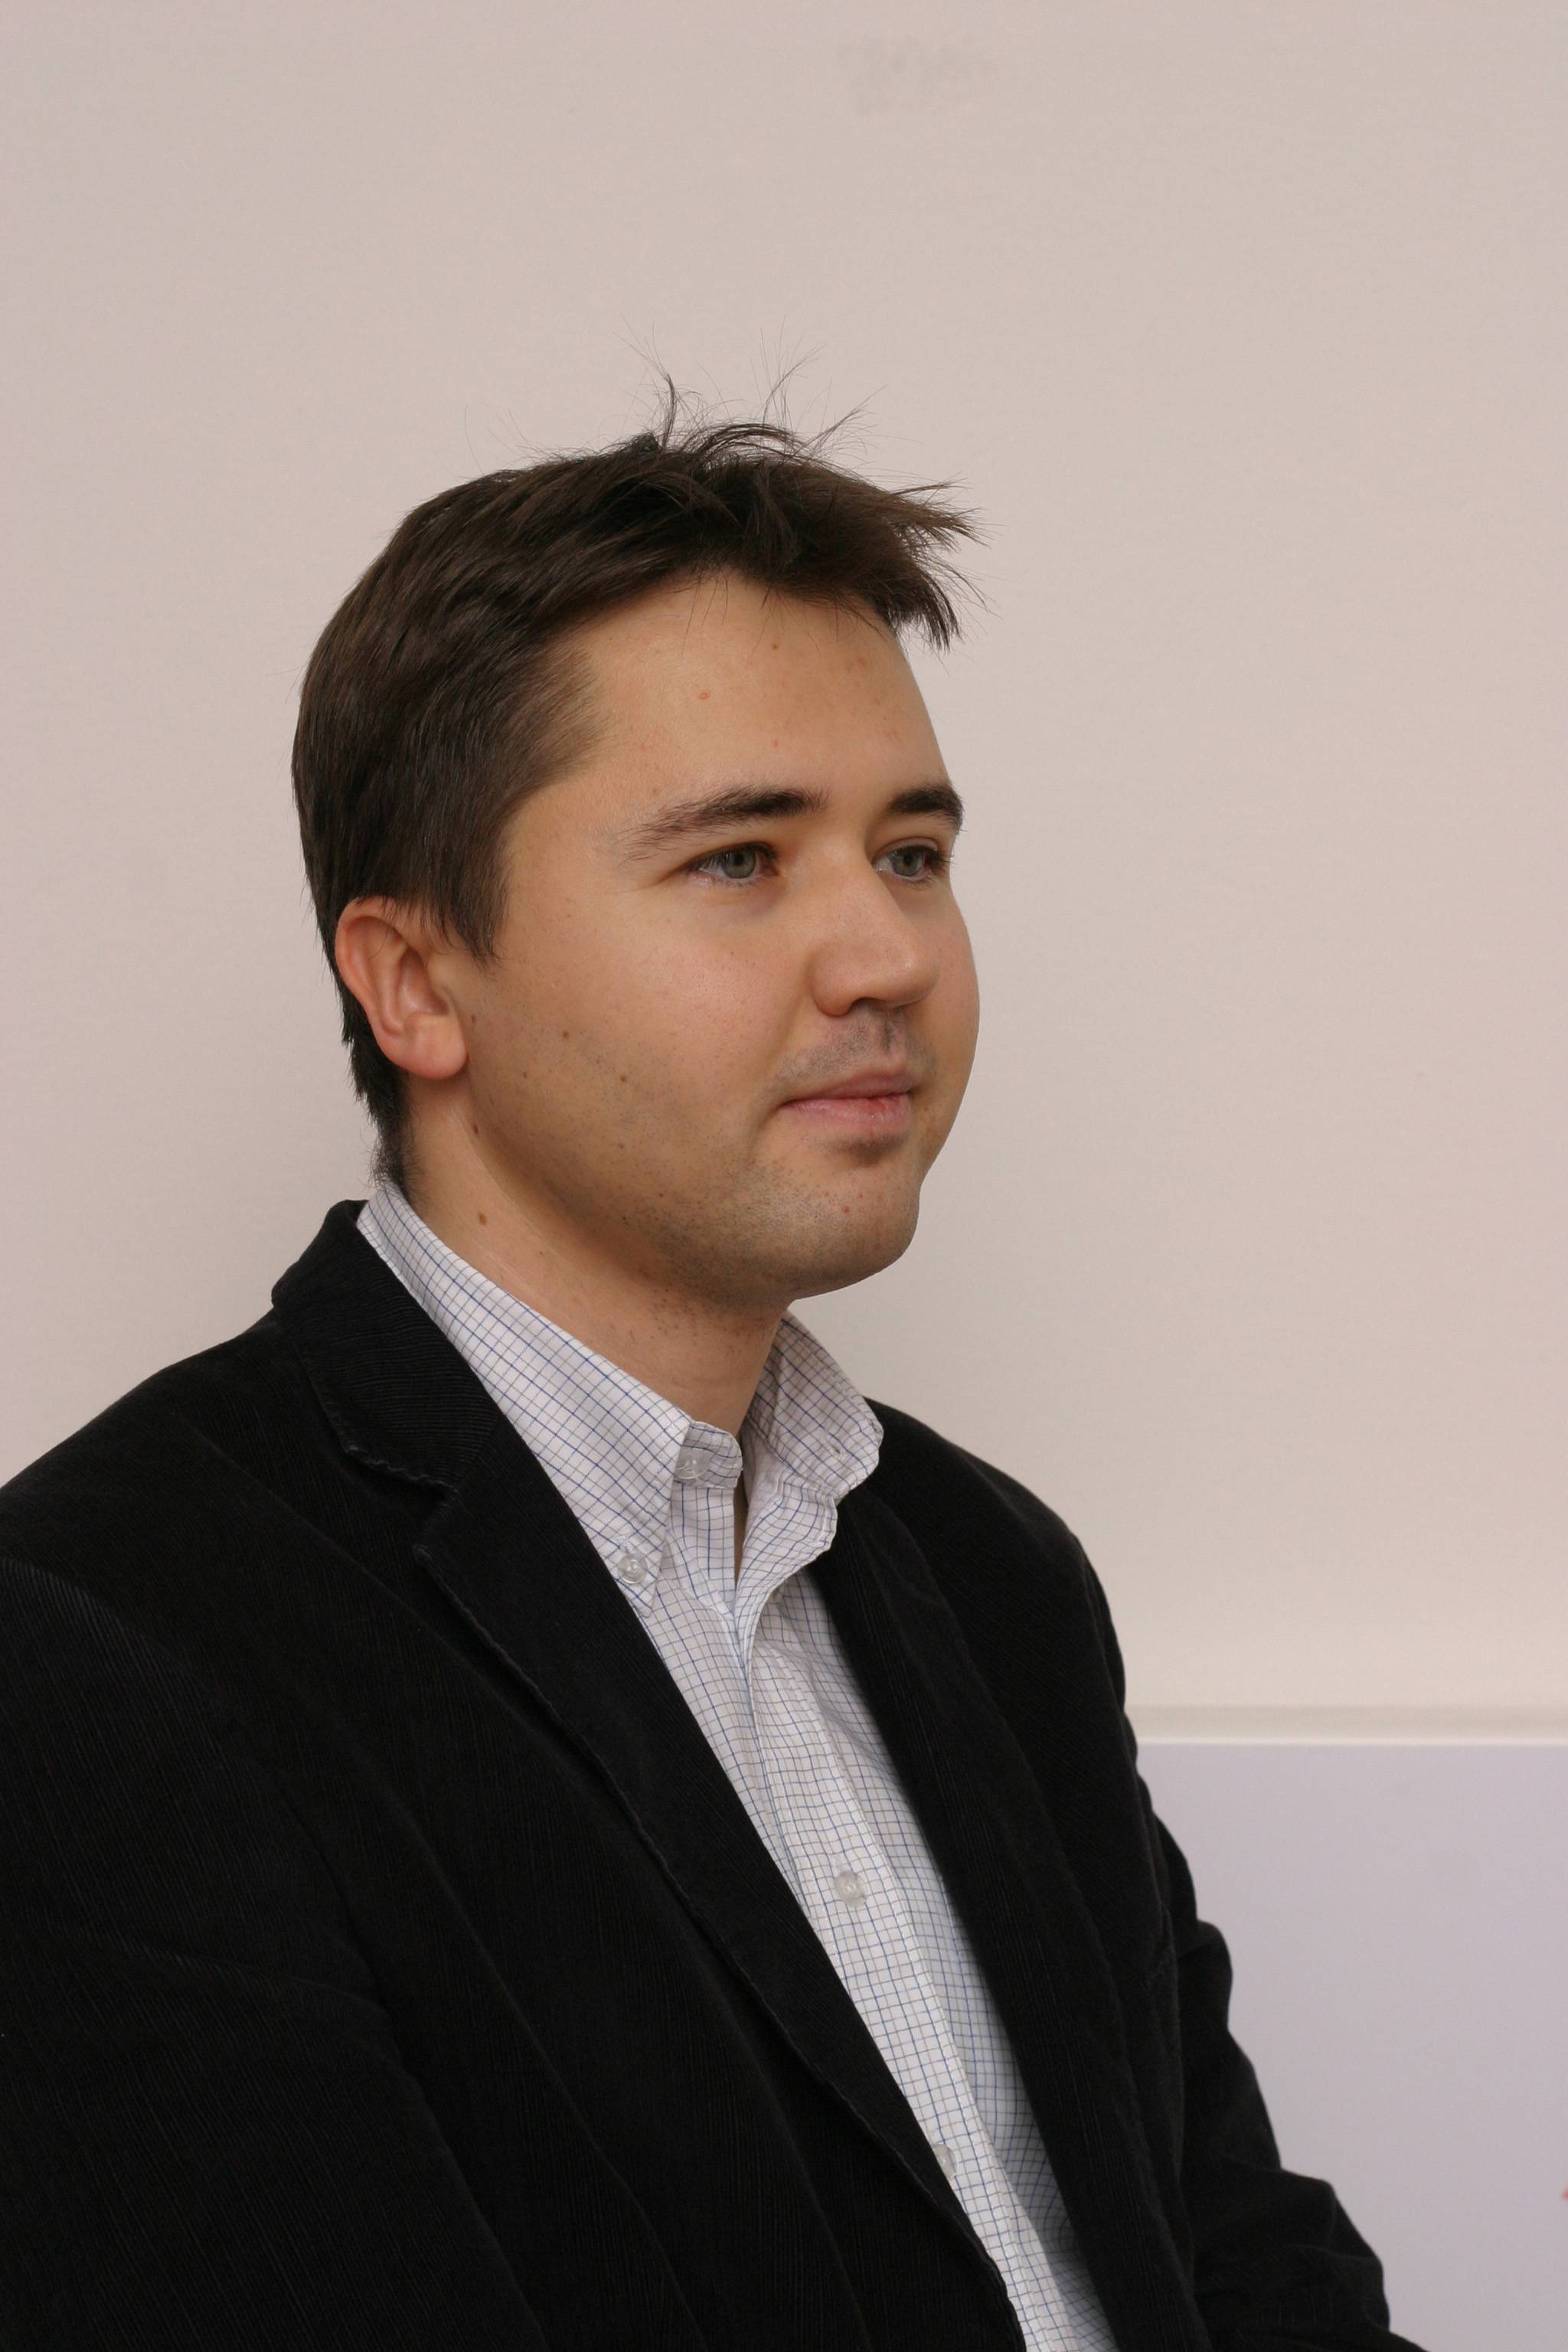
\includegraphics[width=0.7in]{d4.jpg} 
   \end{minipage}
   \begin{minipage}[t]{0.18\linewidth} 
     \centering 
     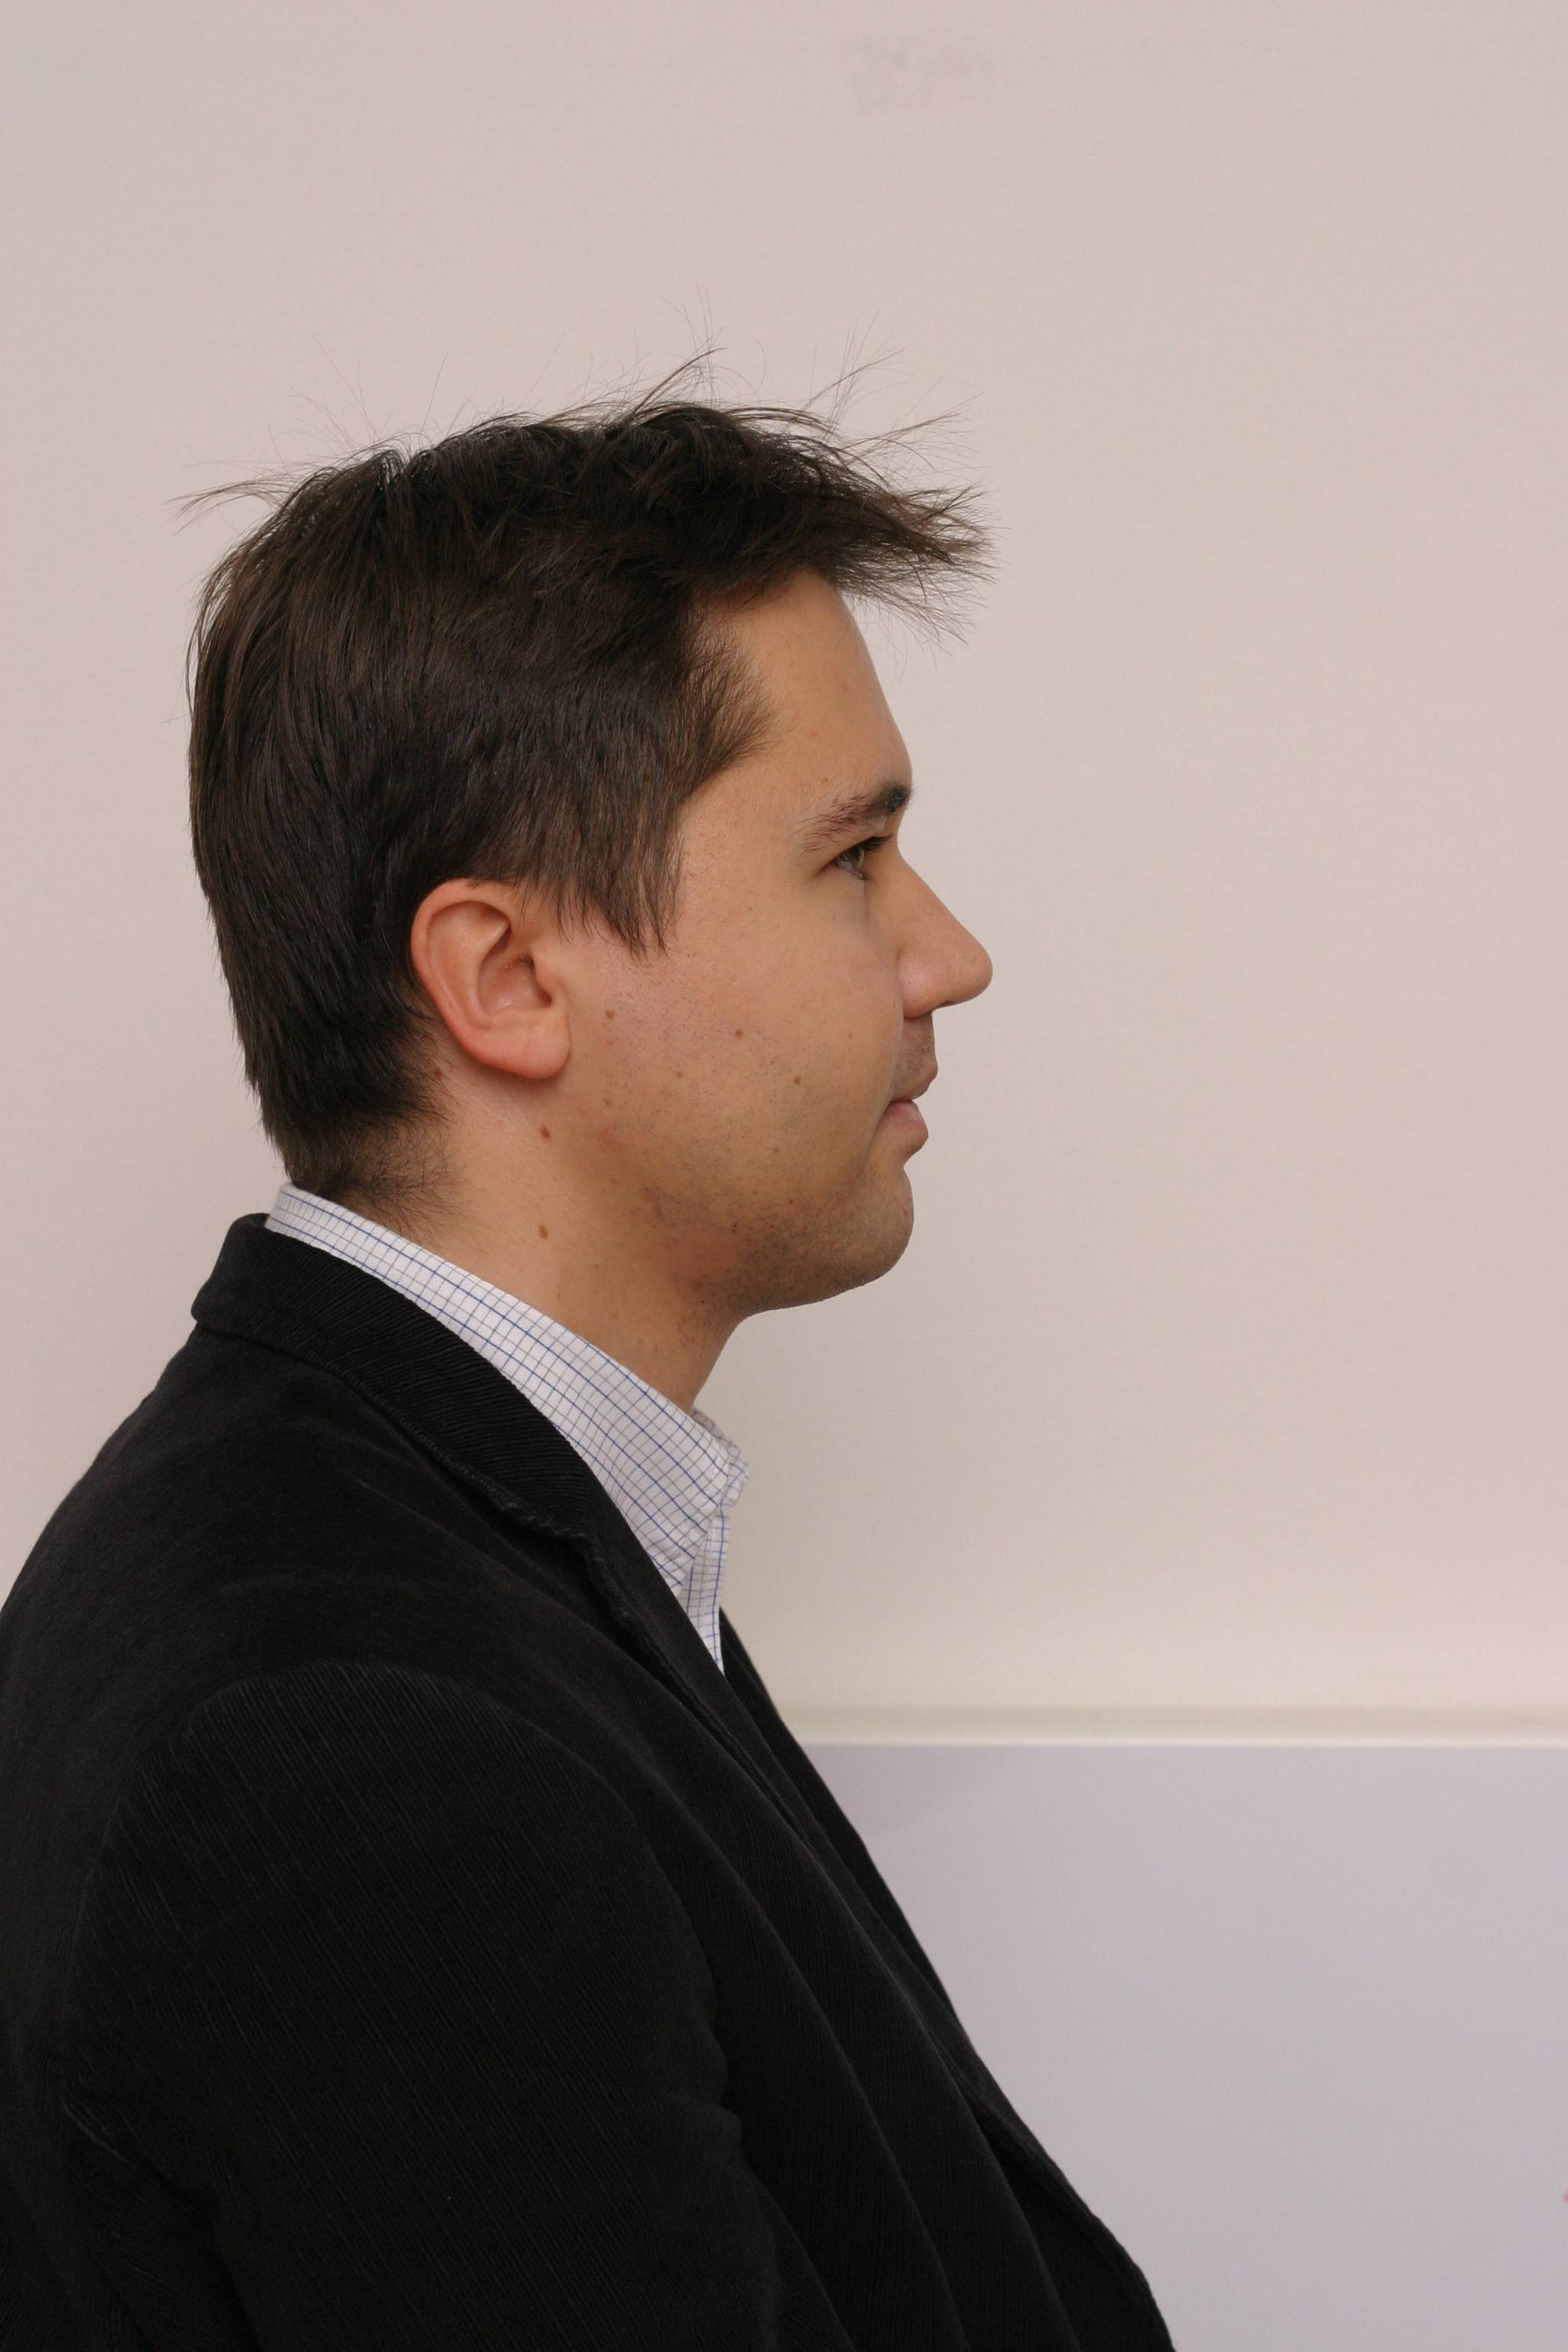
\includegraphics[width=0.7in]{d5.jpg} 
   \end{minipage}
   \end{figure}
\end{frame}





\begin{frame}
    \frametitle{Challenges}
   \begin{itemize}
   \item Facial Expression\footnote{The yalefaces B Datebase}
   \end{itemize}
     \begin{figure}
     \begin{minipage}[t]{0.35\linewidth} 
     \centering 
     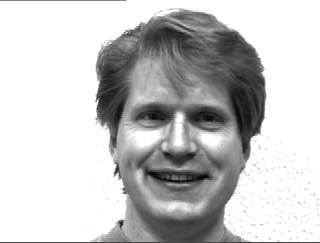
\includegraphics[width=1.35in]{happy.jpg} 
   \end{minipage}
   \begin{minipage}[t]{0.35\linewidth} 
     \centering 
     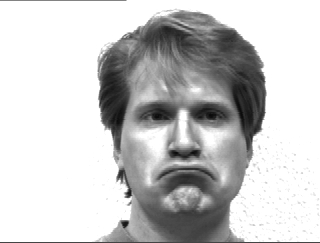
\includegraphics[width=1.35in]{sad.jpg} 
   \end{minipage} 
   \begin{minipage}[b]{0.35\linewidth} 
     \centering 
     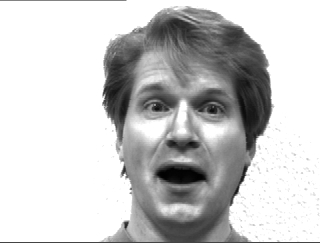
\includegraphics[width=1.35in]{surprise.jpg} 
   \end{minipage}
   \begin{minipage}[b]{0.35\linewidth} 
     \centering 
     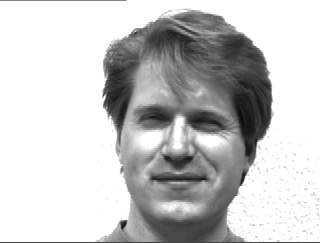
\includegraphics[width=1.35in]{wink.jpg} 
   \end{minipage}
   \end{figure}
\end{frame}



\begin{frame}
    \frametitle{Challenges}
   \begin{itemize}
   \item Occlusion
     \begin{figure}
     \begin{minipage}[t]{0.35\linewidth} 
     \centering 
     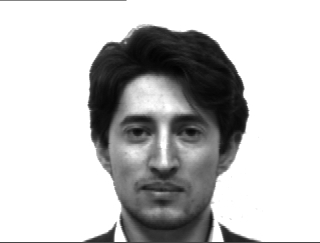
\includegraphics[width=1.4in]{noglass.jpg} 
   \end{minipage}
   \begin{minipage}[t]{0.35\linewidth} 
     \centering 
     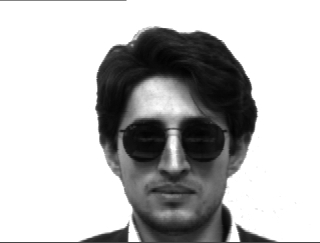
\includegraphics[width=1.4in]{glass.jpg} 
   \end{minipage} 
   \end{figure}
   \end{itemize}
   \begin{itemize}
   \item Imaging Conditions
     \begin{figure}
     \begin{minipage}[t]{0.32\linewidth} 
     \centering 
     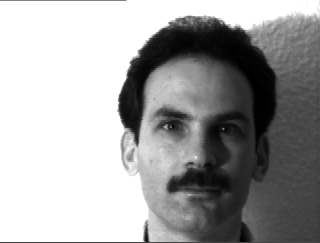
\includegraphics[width=1.4in]{left.jpg} 
   \end{minipage}
   \begin{minipage}[t]{0.32\linewidth} 
     \centering 
     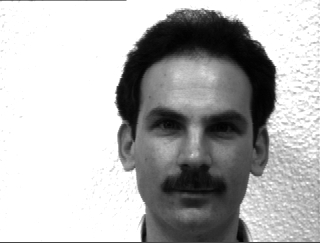
\includegraphics[width=1.4in]{normal.jpg} 
   \end{minipage} 
   \begin{minipage}[t]{0.32\linewidth} 
     \centering 
     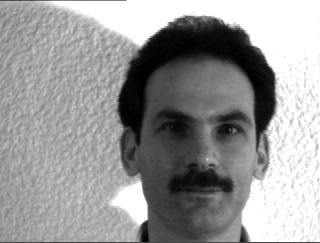
\includegraphics[width=1.4in]{right.jpg} 
   \end{minipage} 
   \end{figure}
   \end{itemize}
\end{frame}

\subsection{Methodology}
\begin{frame}
    \frametitle{Methodology}
   \begin{figure}[!ht]
   \centering
   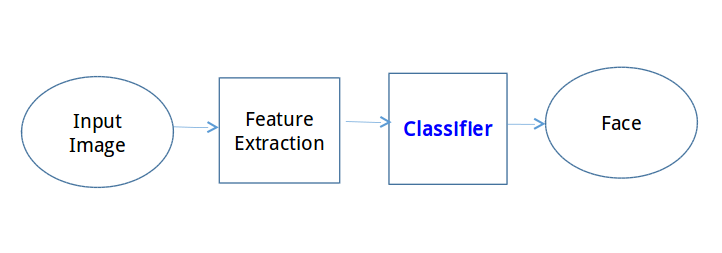
\includegraphics[width=4.0in]{process.png}
   \end{figure}
\end{frame}

\begin{frame}
    \frametitle{Methodology}
   \begin{figure}[!ht]
   \centering
   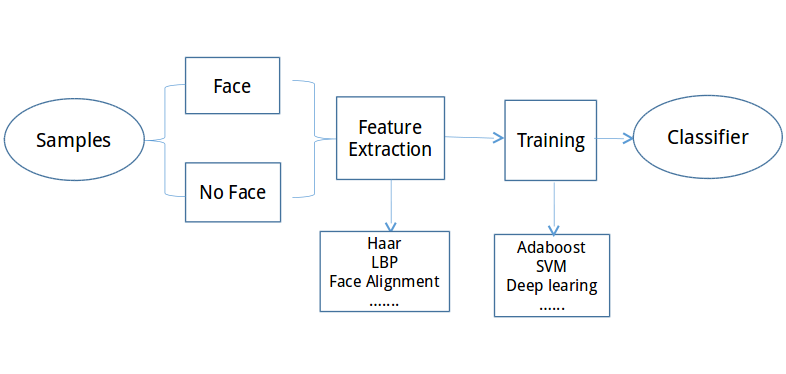
\includegraphics[width=4.0in]{training.png}
   \end{figure}
\end{frame}



\section{Development}

\begin{frame}
    \frametitle{Development}
   \begin{itemize}
   \item Classical Methods
   \item State-of-the-art
   \end{itemize}
\end{frame}


\subsection{Classical Methods}
\begin{frame}
    \frametitle{Classical Methods}
   \begin{itemize}
   \item Knowledge-Based Methods
   \item Feature Invariant Approaches
      \begin{itemize}
      \item Texture
      \item Skin Color
    %  \item Multiple Features
      \end{itemize}
   \item Template Matching Methods
      \begin{itemize}
      \item Predefined Templates
       \item Deformable Templates
       \end{itemize}
   \item Appearance-Based Methods
       \begin{itemize}
%       \item Eigenfaces
    %   \item Distribution-Based Methods
       \item Neural Networks
       \item Support Vector Machines
    %  \item Sparse Network of Winnows
     %  \item Naive Bayes Classifier
     %  \item Hidden Markov Model
       \item Information-Theoretical Approach
     %  \item Inductive Learning
       \end{itemize}
   \end{itemize}        
\end{frame}


\subsection{State-of-the-art}
\begin{frame}
    \frametitle{State-of-the-art}
    \begin{enumerate}
   \item Real-Adaboost\footnote{ "Efficient Boosted Exemplar-based Face Detection". Haoxiang Li, Zhe Lin, Jonathan Brandt, Xiaohui Shen, Gang Hua, CVPR, 2014}\\
 %  \item Sparse Representation:"Robust Face Recognition via Sparse Representation". John Wright,Allen Y. Yang,Arvind Ganesh,S. Shankar Sastry.PAMI,2009
   \item Sparse Representation \footnote{"Single-Sample Face Recognition with Image Corruption and Misalignment via Sparse Illumination Transfer". Liansheng Zhuang, Allen Y. Yang, Zihan Zhou, S. Shankar Sastry, and Yi Ma.CVPR,2013}
%   \item "Neither Global Nor Local: Regularized Patch-Based Representation for Single Sample Per Person Face Recognition". Shenghua Gao, Kui Jia, Liansheng Zhuang, Yi Ma, IJCV, 2014
   \end{enumerate} 
\end{frame}

\section{Haar-Classifier}
\begin{frame}
    \frametitle{Haar-Classifier}   
   Viola-Jones Face Detector\footnote{P Viola,M Jones, "Robust Real-Time Face Detection", IJCV, 2004}: \newline
 Haar + Integral Image + \textbf{Classifier} + Cascade  \newline
   \begin{figure}[!ht]
   \centering
   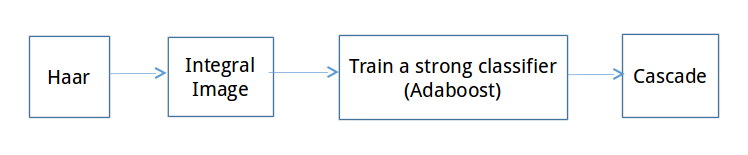
\includegraphics[width=4.1in]{detector.png}
   \end{figure}
\end{frame}

\subsection{Haar}  
\begin{frame}
    \frametitle{Haar}   
   \begin{itemize}
   \item Edge features\footnote{CP Papageorgiou \textit{et al.}, "A general framework for object detection", ICCV, 1998}
   \begin{figure}[!ht]
   \centering
   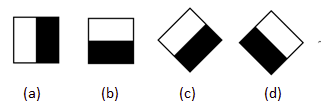
\includegraphics[width=1.4in]{h1.png}
   \end{figure}
   \item Lines features
   \begin{figure}[!ht]
   \centering
   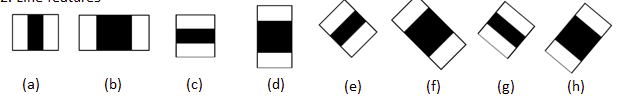
\includegraphics[width=3.0in]{h2.png}
   \end{figure}
   \item Center-Surround features
   \begin{figure}[!ht]
   \centering
   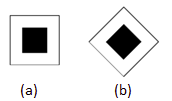
\includegraphics[width=0.9in]{h3.png}
   \end{figure}
   \end{itemize}   
\end{frame}

\begin{frame}
    \frametitle{Haar} 
   \begin{figure}[!ht]
   \centering
   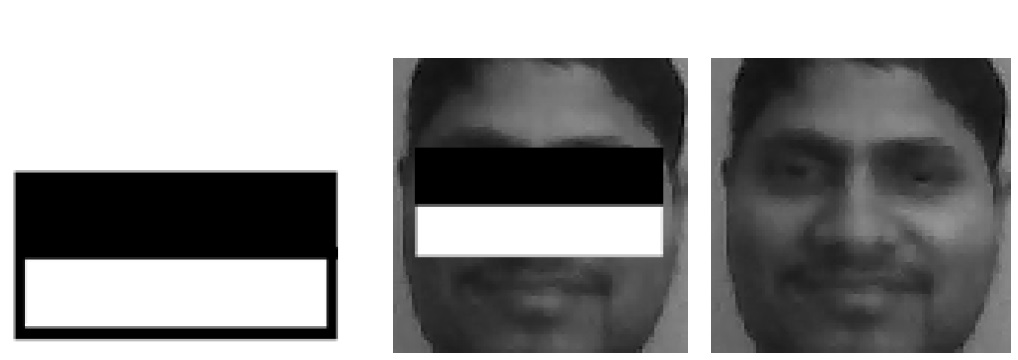
\includegraphics[width=2.8in]{haar1.jpg}
   \end{figure}
   \begin{figure}[!ht]
   \centering
   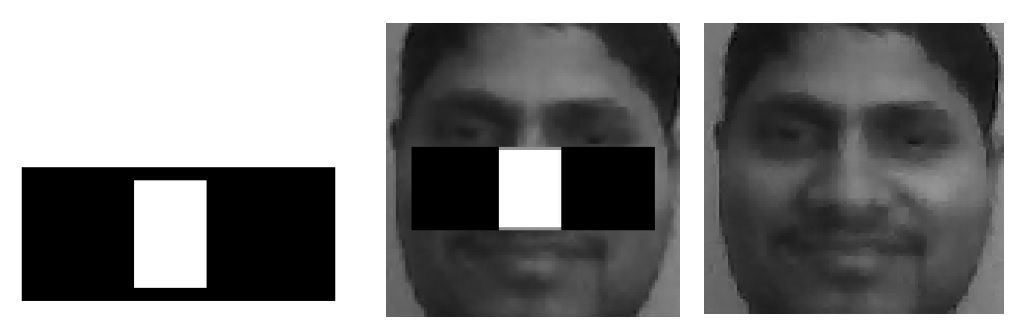
\includegraphics[width=2.8in]{haar2.jpg}
   \end{figure}
\end{frame}

\subsection{Adaboost}
\begin{frame}
    \frametitle{Adaboost}
    \begin{itemize}
 %  \item PAC (Probably Approximately Correct) Model 
   \item Boosting
   \item Adaboost(adaptive boosting)
   \end{itemize} 
\end{frame}


\begin{frame}
    \frametitle{Boosting}
   \begin{itemize}
 \item Weak learning\footnote{L, G. VALIANT, "A Theory of the Learnable", ACM, 1984}
 \item Strong learning
  \item Weak Classification $\longrightarrow$  Stronger Classifier\footnote{MJ Kearns, "The Computational Complexity of Machine Learning", ACM, 1990}
  \end{itemize}
 \end{frame}


\begin{frame}
   \frametitle{Boosting}
   \begin{itemize}
   \item Weak Classifier\footnote{Y Freund, RE Schapire, "A Decision-Theoretic Generalization of On-Line Learning and an Application to Boosting", J COMPUT SYST SCI, 1997}
   \end{itemize}
   \begin{displaymath}
   f(x,f,p, \theta ) = \left \{ \begin{array}{ll}
   1 & \textrm{ $ pf(x)>p\theta $ }\\
   0 & \textrm{other} 
    \end{array} \right.
   \end{displaymath}
   \begin{figure}[!ht]
   \centering
   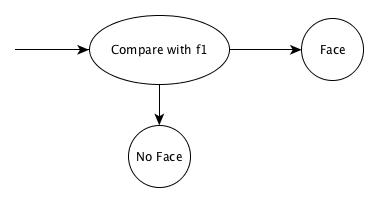
\includegraphics[width=2.6in]{classifier.jpg}
   \end{figure}
\end{frame}


\begin{frame}
    \frametitle{Boosting}
   \begin{itemize}
   \item Strong Classifier
   \end{itemize}

   \begin{figure}[!ht]
   \centering
   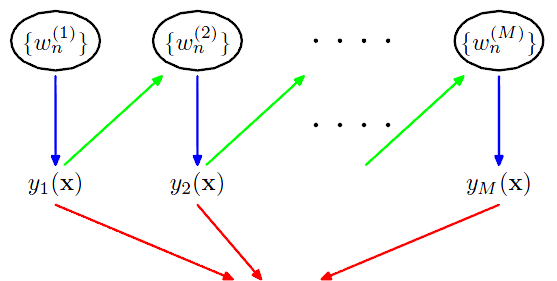
\includegraphics[width=3.5in]{AAUgraphics/yx.png}
   \end{figure}
   \begin{figure}[!ht]
   \centering
   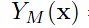
\includegraphics[width=0.8in]{AAUgraphics/yx1.png}
   \end{figure}

 %  \begin{displaymath}
 %  C(x) = \left \{ \begin{array}{ll}
 %  1 & \textrm{$ \sum_{t=1}^T \alpha_t h_t(x) \geq  \frac{1}{2} \sum_{t=1}^T \alpha_t $} \\
 %  0 & \textrm{other} 
 %   \end{array} \right.
 %  \end{displaymath}
\end{frame}


\begin{frame}
    \frametitle{Adaboost}
   \footnote{Y Freund, RE Schapire, "A Decision-Theoretic Generalization of On-Line Learning and an Application to Boosting", J COMPUT SYST SCI, 1997}
   \begin{figure}[!ht]
   \centering
   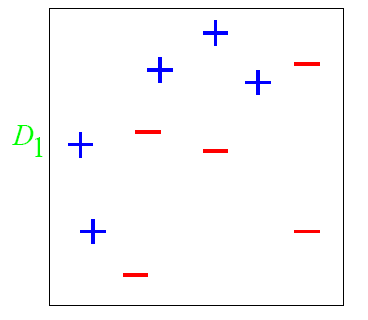
\includegraphics[width=2.0in]{AAUgraphics/ada1.png}
   \end{figure}
\end{frame}



\begin{frame}
    \frametitle{Adaboost}
   \begin{figure}[!ht]
   \centering
   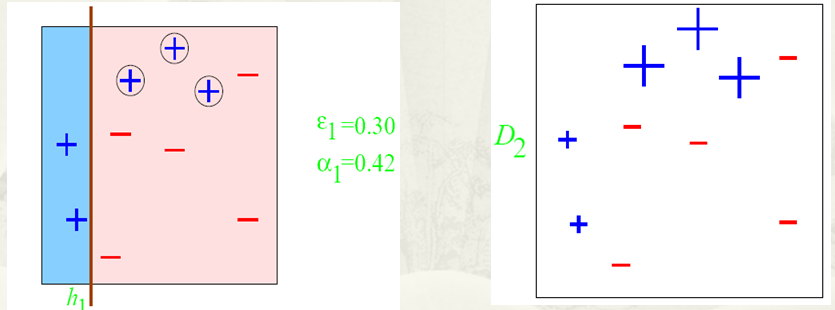
\includegraphics[width=3.0in]{AAUgraphics/ada2.png}
   \end{figure}
   \begin{figure}[!ht]
   \centering
   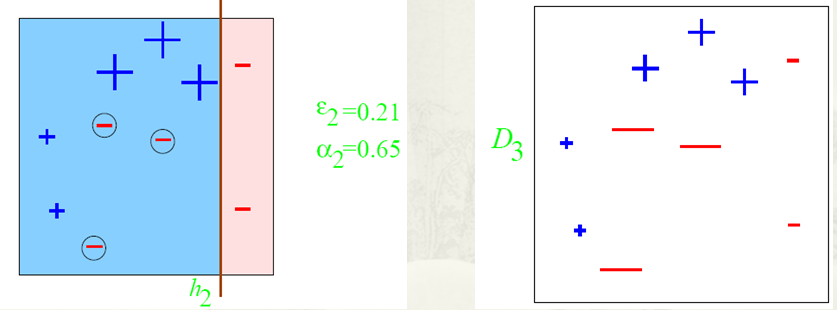
\includegraphics[width=3.0in]{AAUgraphics/ada3.png}
   \end{figure}
\end{frame}


\begin{frame}
    \frametitle{Adaboost}
   \begin{figure}[!ht]
   \centering
   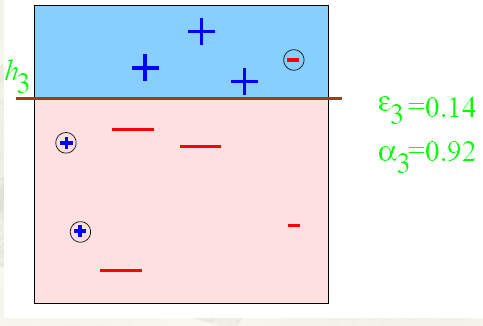
\includegraphics[width=2.2in]{AAUgraphics/ada4.png}
   \end{figure}
\end{frame}

\begin{frame}
    \frametitle{Adaboost}
   \begin{figure}[!ht]
   \centering
   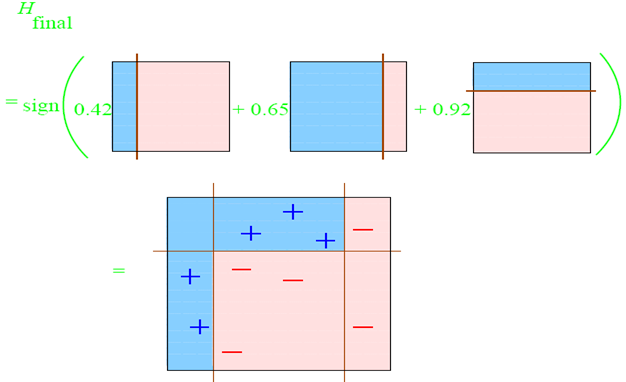
\includegraphics[width=3.2in]{AAUgraphics/ada5.png}
   \end{figure}
\end{frame}


\begin{frame}
    \frametitle{Adaboost}
   \large Output the final hypothesis:
   \begin{displaymath}
   H(x) = sign(\sum_{t=1}^T  \alpha_t h_t(x))  
   \end{displaymath}
   \newline
   \large Weight:
   \newline
   \begin{displaymath}
   \alpha_t =  \frac{1}{2} ln (\frac{1-\varepsilon_t}{\varepsilon_t})
   \end{displaymath}
\end{frame}



\subsection{Cascade}
\begin{frame}
   \frametitle{Cascade}
   \begin{figure}[!ht]
   \centering
   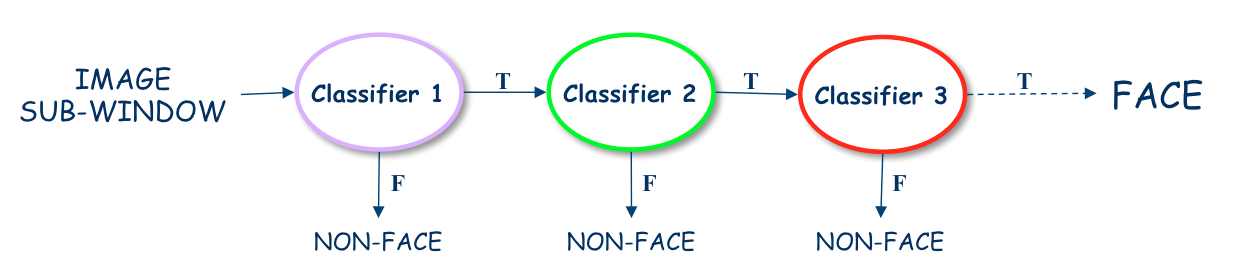
\includegraphics[width=4.0in]{AAUgraphics/liucheng.png}
   \end{figure}
\end{frame}


{\aauwavesbg
\begin{frame}[plain,noframenumbering]
  \finalpage{\huge Thank You Very Much}
\end{frame}}

\end{document}
